\chapter{An Introduction to Gaussian Processes by
\href{http://learning.eng.cam.ac.uk/Public/Turner/WebHome}{Richard Turner}}

Example with a non-linear regression

Start with an example of a multivariate Gaussian

\begin{equation}
  p(y|\Sigma) \propto  \exp (\frac{-1}{2} y^T \Sigma^{-1}y)
\end{equation}

If we condition the probabilities of one variable we obtain Gaussian shaped
distributions as well


\begin{equation}
  p(y_2 | y_1, \Sigma) \propto (\exp (\frac{-1}{2} y^T (y_2 - \mu_0)\Sigma^{-1}y(y_2 - \mu_0))
\end{equation}

TODO: revise previous equation

If we map any sample from the original distribution, it is possible to draw a
line with the x-axis the different variables (variable index), and the y-axis the coordinates.
If the variables are correlated, the lines should be quite horizontal.

In the examples it goes from 2 variables to 20, and show how the farther is the
variable less correlated is to the first variable.

In the example, there is a coviariance matrix with a Gaussian with fixed
variance in the diagonal with the mean going from the first variable to the
last one.

Then, if some of this variables are actual samples (fix values), then the
sampling process should force the other variables to converge to these samples.
(TODO: check if the following equation is an ``l'' or an ``I'')

\begin{align}
  \Sigma(x_1, x_2) = \Kernel(x_1, x_2) + l\sigma_y^2 \\
  \Kernel(x_1, x_2) = \sigma^2e^{-\frac{1}{2l^2}(x_1 - x_2)^2}
\end{align}

I a non-parametric method  (infinit parameters)

\begin{align}
  p(y|\theta) = \Normal(y;0,\Sigma) \\
\end{align}

where $\sigma^2$ is the scale (vertical scale), and $l$ is the horizontal-scale
(this scales can be seen in the previous lineplot).

In a parametric model

\begin{align}
  y(x) = f(x;\theta) + \sigma_y \epsilon \\
  \epsilon \from \Normal(0,1)
\end{align}

Definition of a Gaussian process: generalisation of a multivariate Gaussian
distribution to infinitely many variables

A Gaussian distribution is fully specified by a mean vector, $\mu$ and a
covariance matrix $\Sigma$.

\begin{equation}
  f = (f_1, \dots, f_n) \from \Normal(\mu, \Sigma) \text{, indices } i=1,
  \dots, n
\end{equation}

\begin{align}
  y(x) = f(x) + \epsilon \sigma_y \\
  p(\epsilon) = \Normal(\epsilon; 0, 1)
\end{align}

place a GP prior over the non-linear function

\begin{align}
  p(f(x)|\theta) = GP(f(x); 0, K_\theta(x,x')) \\
  \Kernel(x, x') = \sigma^2 \exp \left( - \frac{1}{2l^2} (x - x')^2\right)
\end{align}

sum of a Gaussian variable into a GP is still a multivariate gaussian.

\begin{equation}
  \text{missing equation}
\end{equation}

The marginalisation property of Gaussian distributions is

\begin{align}
  p(y_1) = \int p(y_1, y_2) dy_2 \\
  p(y_1, y_2) = \Normal \left( \left[ \right] \text{missing} \right) \rightarrow p(y_1) =
  \Normal(y_1: a, A)
\end{align}

How do twe make a prediction

\begin{align}
  p(y_1 | y_2) = \frac{p(y_1, y_2)}{p(y_2)} \\
  \rightarrow p(y_1|y_2) = \Normal(y_1: a + BC^{-1} (y_2 - b), A - BC^{-1}B^T)
\end{align}

Where $y_1$ are the predicted positions and $y_1$ are the samples

The predictive mean (first part of $\Normal$ is linear in the data $=Wy_2$

The predictive covariance (second part of the $\Normal$) ca be interpreted as
the predictive uncertanity = prior uncertainty $A$ - the reduction in
uncertainty $BC^{-1}B^T$.

What are the implications of the hyper-parameters?

\begin{itemize}
  \item $\sigma$ missing implications
  \item $l$ missing implications
\end{itemize}

We can use the probability distributions to represent the plausibility of the
hyper-parameters (uncertainty) given the data

\begin{equation}
  \text{Bayes theorem with posterior probability of data given the parameters}
\end{equation}

Shows an example of modifying the lengh-scale variable $l$ and showing how the
likelihood of the parameter value starts increasing and decreasing, showing a
peak at lenghtscale 2.

\newcommand\gauss[2]{1/(#2*sqrt(2*pi))*exp(-((x-#1)^2)/(2*#2^2))} % Gauss function, parameters mu and sigma

\begin{figure}[h]
  \centering
  \begin{tikzpicture}
  \begin{axis}[every axis plot post/.append style={
      mark=none,domain=-2:10,samples=50,smooth},
  ylabel=likelihood,
  xlabel=lenght-scale,
  width=\linewidth,
  height=5cm,
  axis x line*=bottom, % no box around the plot, only x and y axis
  axis y line*=left, % the * suppresses the arrow tips
  enlargelimits=upper] % extend the axes a bit to the right and top
  \addplot {\gauss{2}{1.2}};
  \end{axis}
  \end{tikzpicture}
  \caption{Likelihood of the data guiven the value of the lenght-scale $l$}
\end{figure}

\section{Covariance functions}

Warning. Difficult to compare different models. If you try to compute the posterior
probability of the different models guiven the data, it is hard to compute, it
needs approximations and the results are really sensitive to the priors.


\subsection{References}

\begin{itemize}
  \item Gaussian Processes for Machine Learning, Rasmussen and Williams, 2006
  \item \href{http://gpss.cc/}{Gaussian Process Summer School}, Neil Lawrence and collegues
    \item Software
      \begin{itemize}
        \item GPy: Gaussian processes in Python
        \item GPflow: Gaussian Processes and tensorflow
        \item GPML: Gaussian Processes in Matlab
        \item GP Stan: Gaussian Processes in probabilistic programming
      \end{itemize}
\end{itemize}

\section{Using Gaussian Processes: Models, applications and connections
16:30--18:00}

Question 1: Addition of two GPs

\begin{align}
  f(x) = f_1(x) + f_2(x) \\
  f_1(x) \from GP(0, \Sigma_1(x,x')) \\
  f_2(x) \from GP(0, \Sigma_2(x,x'))
\end{align}

The expected value is

\begin{align}
  m(x) = \Expected(f(x)) =& \Expected(f_1(x) + f_2(x)) \\
  =& \Expected(f_1(x)) + \Expected(f_2(x))
\end{align}

And the covariance is

\begin{align}
\Sigma(x) =& \Expected(f(x)f(x')) - \Expected(f(x))\Expected(f(x)) \\
=& \Expected\left[\left(f_1(x) + f_2(x'))(f_1(x) + f_2(x')\right)\right] \\
=& \Expected[f_1(x) + f_1(x')] + \Expected[(f_2(x) + f_2(x')] + \Expected[f_1(x) + f_2(x')] + \Expected[(f_2(x) + f_1(x')] \\
=& \Expected[f_1(x) + f_1(x')] + \Expected[(f_2(x) + f_2(x')]
\end{align}

More generally: GPs closed under linear transofmration / combination:

\begin{itemize}
  \item GP multiplied by a deterministic function = GP
  \item derivatives of GP = GP
  \item integral of a GP = GP
  \item convolution of a GP by a deterministic funtion = GP
\end{itemize}

Question 2: Random linear model

\begin{align}
  g(x) = mx + c \\
  m \from \Normal(0, \sigma_m^2) \\
  c \from \Normal(0, \sigma_c^2)
\end{align}

The expected value

\begin{equation}
  m(x) = \Expected[g(x)] = \Expected(m)x + \Expected(c) = 0 + 0
\end{equation}

The covariance

\begin{align}
  \Sigma(x, x') =& \sigma_m^2 xx' + \sigma_c^2 \\
  =& \Expected(g(x)g(x')) \\
=& \Expected(( mx + c)(mx' + c)) \\
=& \Expected(m^2)xx' + \Expected(c^2) + \Expected(cm)x' + \Expected(mc)x \\
=& \Expected(m^2)xx' + \Expected(c^2) + 0 + 0
\end{align}

Question 3: random sinusoid model

\begin{align}
  h(x) = a \cos(wt) + b \sin(wt) \\
  a \from Normal(0, \sigma^2) \\
  b \from Normal(0, \sigma^2)
\end{align}

\begin{equation}
  m(x) = 0
\end{equation}

\begin{equation}
  \Sigma(x,x') = \sigma^2\cos(w(x-x'))
\end{equation}

Bochner's theorem: Any stationary covariance function can be written as

\begin{equation}
  \Sigma(x - x') = \int \sigma^2 (x) \cos(w(x-x'))dw
\end{equation}

roughly, the function comprises and uncontably infinite sum of random sins and
cosines


\begin{table}[h]
  \def\arraystretch{2.0}
  \centering
  \begin{tabular}{p{.3\linewidth}|p{.3\linewidth}|p{.3\linewidth}}
    linear mappings $f(x) = Wx$ & neural network & Gaussian Process mappings \\
    \hline
    linear regression & neural network regression & Gaussian Process regression \\
    PCA or Factor analysis & variational auto-encoder (VAE) & Gaussian Process latent variable model \\
    Gaussian auto-regressive (or Markov) model & neural auto-regressive density estimation (NADE) & Gaussian process auto-regressive model (GPAR) \\
    linear Gaussian state space model (LGSSM) & recurrent neural latent variable model & Gaussian process state-space model (GP-SSM)
  \end{tabular}
\end{table}

Strenghts of Gaussian Processes

\begin{itemize}
  \item Interpretable machine learning
  \item data-efficient machine learning
  \item decision making
  \item automated machine learning including probabilistic numerics
\end{itemize}

Weaknesses

\begin{itemize}
  \item Large numbers of datapoints ($N \le 10^5$)
  \item High-dimensional inputs spaces ($D \le 10^2$)
\end{itemize}

In the speakers opinion, GPs are not good for large image recognition tasks,
but for small tasks where it is cruciall to get uncertainty estimates.

Example of an Interpretable \href{https://cloud.google.com/automl/}{auto-ML}: the automatic statistician

Given some airline data it detects four underlying patterns, linearly
increasing factor, a periodicity at every year, some incresing noise.

Shows an example with a video of an inverted pendulum and how in a small number
of iterations (around 7?) a GP is learned.

\subsection{Deep Gaussian Processes}

Allowing non-parametric kernel spaces

\begin{align}
  y(x) = f(x) + \sigma_y \epsilon \\
  \text{missing this part}
\end{align}

with a composition of GPs

\begin{align}
  y(x) = f(g(x)) + \sigma_y \epsilon \\
  f(x) = GP(0, K_f(x,x')) \\
  g(x) = GP(0,K_g(x,x'))
\end{align}

Deep GP may perform automatic kernel design


A Neural Network with one hidden layer and infinite number of units in the
hidden layer is a Gaussian Process Nial 1996

A Neural Network  with multiple hidden layers with infinite number of hidden
units on each layer is also a GP (the variance on the weights need a specific
  variance $\sigma^2/D$ Matthews et al. 2018. The specific variance is the
  reason why with finite number of units the regularisation needs to be
  readjusted and follows the values found by Matheews et al.

\subsection{References}

\begin{itemize}
  \item Gaussian process latent variable models for visualisation of high
    dimensional data by Lawrence
  \item Local distance preservation in the GP-LVM throught Back constraints
  \item the automatic statistician
  \item PILCO: a model-based and data-efficient approach to policy serch
\end{itemize}

\section{Large data and non-linear models Tue. 11:30--13:00}

Shows a few examples of sounds generation using Gaussian Processes.

\section{A brief history of gaussian process approximation}

One of the first approaches was to modify the original samples in a way that
the computational complexity of making exact inference was reduced from $O(n^3$
to $O(n^2)$.

See following publications:

\begin{itemize}
  \item Sparse Gaussian Processes using Pseudo-inputs
  \item Local and global sparse gaussian process approximations
  \item Sparse-posterior Gaussian Processes for general likelihoods
  \item Variational Learning of Inducing variables in sparrse Gaussian
    Processes
  \item Fast Forward selection to speed up sparse Gaussian Process Regression
\end{itemize}

Some examples of Factor graphs

\begin{align}
  p(x_1, x_2, x_3) = g(x_1, x_2, x_3) \\
  p(x_1, x_2, x_3) = g_1(x_1, x_2)g_2(x_2, x_3) \\
\end{align}

Where in the first one all the nodes are connected with one factor (square),
while the second one $x_1$ is only connected to $x_2$ and this one to $x_3$.

Shows an example of a multivariate gaussian where the covariance matrix has
some numbers, and the inverse of the covariance matrix presents some zeros. By
looking at the inverse of the covariance matrix we can see what nodes are
independent guiven the rest (positions whith the value zero).

\begin{align}
  \Normal(x, \mu, \Sigma) \propto& \exp[-1/2 (x- \mu)^T \Sigma^{-1}(x- \mu)] \\
  =& \exp[-1/2 \sum_{i,j}(x_i - \mu_i)\Sigma_{i,j}^{-1}(x_j - \mu_j)] \\
  =& \prod_{i,j} \exp[-1/2 (x_i - \mu_i)\Sigma_{i,j}^{-1}(x_j - \mu_j)] \\
  =& \prod_{i,j} g_{i,j}(x_i, x_j)
\end{align}

The previous equations show that when the inverse of the covariance is 0, the
exponent value goes to one and the multiplicative factors are not affected.


The Kullback-Leibler divergence has the Gibb's inequality property, that means
that $KL(p_1(z) || p_2(z)) \ge 0$ and has the equality at $p_1(z) = p_2(z)$. In
order to prove the previous property apply the Jensen's inequality or
differentiation. It is also Non-symmetric $KL(p_1(z) || p_2(z)) \ne
KL(p_2(z) || p_1(z))$.

\subsection{Fully independent training conditional (FITC) approximation}

\begin{enumerate}
  \item Augment model with $M < T$ pseudo data
    \begin{equation}
      p(f, u) = \Normal(\text{f u, with mean 0 and covariance K})
    \end{equation}
  \item Remove some of the dependencies (results in a simpler model)
  \item Calibrate model (e.g. using KL divergence, many choices)
\end{enumerate}

\begin{itemize}
  \item This method introduces a pareametric bottleneck into a non-parametric
    model
  \item Should we add extra pseudo-data when more data is avilable?
\end{itemize}

\subsection{Variational free-energy method (VFE)}

In this case we want to lower bound the likelihood

\begin{align}
  \Likelihood(\theta) =& \log p(y|\theta) = \log \int df p(y,f|\theta) \\
  =& \log \int df p(y, f|\theta) \frac{q(f)}{q(f)} \ge \int dfq(f) \log
  \frac{p(y,f|\theta)}{q(f)} = F(\theta) \\
  =& \int dfq(f) \log \frac{p(f|y,\theta)p(y|\theta)}{q(f)} = \log p(y|\theta)
  - \KL(q(f)||p(f|y))
\end{align}

\begin{align}
  F(\theta) = \int dfq(f) \log \frac{p(y,f|\theta)}{\text{missing}}
\end{align}

At the end we get a lower bound of the likelihood.

\begin{align}
  F(\theta) =& \int dfq(f) \log \frac{p(y,f|\theta)}{p(f_{\ne u}|u)q(u)} \\
  =& \int dfq(f) \log \frac{p(y|f,\theta)p(f_{\ne u}|u)p(u)}{p(f_{\ne u}|u)q(u)} \\
  =& \int dfq(f) \log \frac{p(y|f,\theta)p(u)}{q(u)}
\end{align}


\begin{figure}[h]
  \centering
  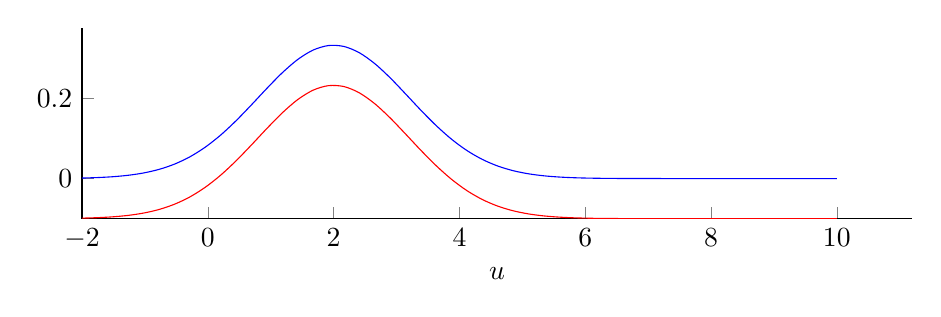
\begin{tikzpicture}
  \begin{axis}[every axis plot post/.append style={
      mark=none,domain=-2:10,samples=50,smooth},
  xlabel=$u$,
  width=\linewidth,
  height=4cm,
  axis x line*=bottom, % no box around the plot, only x and y axis
  axis y line*=left, % the * suppresses the arrow tips
  enlargelimits=upper] % extend the axes a bit to the right and top
  \addplot {\gauss{2}{1.2}};
  \addplot {\gauss{2}{1.2}-0.1};
  \end{axis}
  \end{tikzpicture}
  \caption{Where the {\color{blue}blue line} is the true likelihood and the
    {\color{red}red} line is the approximated $q(u)$}
\end{figure}

They may reduce the time complexity from $O(M^3)$ to $O(NM^2)$, however $N$ is
porportional to $M$ and in certain way is just a small improvement.

Some extra references about approximate inference in GPs:

\begin{itemize}
  \item Sparse online gaussian processes
  \item A unifying view of sparse approximate gaussian process regression
  \item variational learning of inducing variables in sparse gaussian processes
  \item on sparse variational methods and the kullback-leibler divergence
    between stochastic processes
  \item A unifying framework for Gaussian Process Pseudo-Point approximation
    using Power Expectation propagation
  \item Streaming sparse gaussian process aproximations
  \item Efficient deterministic approximate Bayesian Inference for Gaussian
    Process Models
\end{itemize}


and about Deep Gaussian processes:

\begin{itemize}
  \item Deep gaussian processes for regression using approximate expectation
    propagation
  \item Doubly stochastic variational inference for deep gaussian processes
\end{itemize}
%\section{Using GPs: Models applications and connections}

%\section{GPs for large data and non-linear models}
